\documentclass[a4paper]{article}
\usepackage{geometry}
\usepackage{listings}
\usepackage{hyperref}
\usepackage{plantuml}
\usetikzlibrary{arrows, shapes, automata, petri, positioning, calc}
\usepackage{graphicx}
\usepackage{ragged2e}
\usepackage{color}
\usepackage{xepersian}
\usepackage{subfiles}
\newgeometry{left=1.4cm, right=1.4cm, bottom=2.0cm, top=2.0cm}
\settextfont[Scale=1]{XB Roya}
\renewcommand{\baselinestretch}{1.5}

\begin{document}
\centerline{پایگاه داده پیشرفته}
\centerline{دکتر شجاعی مهر}
\centerline{علیرضا سلطانی نشان}
\centerline{\today}
\tableofcontents

\newpage

\section{تراکنش}

تراکنش واحد اجرای برنامه است. عملیاتی که در هر تراکنش می‌تواند شامل شود موارد
زیر می‌باشد:

\begin{itemize}
    \item Create
    \item Read
    \item Update
    \item Delete
\end{itemize}

\section{قوانین \lr{ACID}}

\subsection{اتمیک یا \lr{Atomicity}}

هر تراکنش دیتابیس به صورت اتمیک می‌باشد. این قضیه بدان معناست که این تراکنش یا
باید کاملا انجام شود یا کلا لغو و صرف نظر شود. در غیر این صورت اگر تراکنش به
صورت ناتمام و ناقص انجام شود عواقب مختلفی روی دیتابیس خواهد گذاشت.

\subsection{جامعیت یا \lr{Consistency}}

هر تراکنش باید از قوانین جامعیت پیروی کند. نمی‌توان داده یا را وارد جدولی از
دیتابیس کرد که به صورت معتبر نباشد. در برخی از مراجع این قانون را به اجرای صحیح
و سازگار تراکنش می‌شناسند. مهم ترین مثال آن است که شما یک \lr{Validation} روی یک
مقداری از فیلد جدول تنظیم می‌کنید که هر داده‌ای بر روی آن فقط با شرایط تعریف شده
بایستی وارد شود.

خالی از لطف نیست که در مورد مرجع پذیری داده‌ها در این قسمت نیز می‌توان صحبت کرد
تا بتواند قوانین جامعیت را به طور صحیح کامل کرد. مرجع پذیری زمانی مطرح می‌شود که
یک رکوردی از داده وقتی وارد جدولی از دیتابیس می‌شود ممکن است ارتباط مشخصی با
جدولی دیگر داشته باشد. پس به همین خاطر کلید‌های اصلی و خارجی در خصوص جامعیت وجود
دارند که داده‌ای معنادار را پس از پرس و جو از دیتابیس به برنامه نویس برگرداند.
یادآوری، بخش جوین‌ها در دیتابیس و تعریف رفرنس در هنگام تعریف کلید جانبی.

\subsection{انزوا یا \lr{Isolation}}

هر سیستم جامع پایگاه داده‌ای باید بتواند روی همروند تراکنش‌ها مدیریت و کنترل
کامل داشته باشد. انزوا تراکنش‌ها قابلیت کنترل و تنظیم بر اساس \lr{DBMS} است.

به طور کل همروندی یا همزمانی به حالتی گفته می‌شود که چند تراکنش بخواهند در یک
زمان به صورت موازی روی یک منبع عملیات خواندن و نوشتن را انجام دهند. اما این
عملیات به طور کل هزینه خاص و مشخصی برای برنامه نویس و مدیر دیتابیس دارد.

\subsection{قابلیت اعتماد یا \lr{Duribility}}

قابلیت اعتماد یکی از مهم‌ترین ویژگی‌های هر سیستم دیتابیسی است. یعنی بتوان
داده‌ها را در پایگاه‌داده به صورت پایدار و ثابت نگهداری و مراقبت کرد. در صورت
بروز مشکل روی داده‌های یک دیتابیس می‌توان به عملیات انجام شده در این قسمت مراجعه
کرد. بطور کلی این بخش قابلیت کنترل و مدیریت دارد و می‌توان مجموعه فرایند‌های
نگهداری و بک‌آپ را به صورت خودکار انجام داد.

\subsection{تنظیم قابلیت انزوا}

انزوا و مدیریت همروندی در دیتابیس به چهار طریق قابل انجام است:

\begin{enumerate}
    \item \lr{Read uncommitted}
    \item \lr{Read commmitted} 
    \item \lr{Repeadable read}
    \item \lr{Serializable}
\end{enumerate}

یادآوری: هر تراکنش دو حالت در پایان پیدا می‌کند:

\begin{itemize}
    \item \lr{Commit}: تراکنش درنهایت تایید و انجام می‌شود
    \item \lr{Abort}: تراکنش در نهایت سقط یا صرفه نظر می‌شود
\end{itemize}

\subsubsection{وضعیت تراکنش}


نکته: \lr{Abort} در دو شرط اتفاق می‌افتد:

\begin{enumerate}
    \item زمانی که اجرای تراکنش به خطای \lr{Run time} دچار شود.
    \item خرابی و نقص سیستم که روی اجرای تراکنش تاثیر می‌گذارد که کامل نشود
\end{enumerate}

\begin{figure}
    \centering
    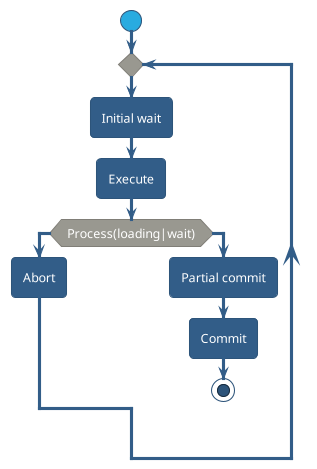
\includegraphics[width=0.5\textwidth]{umls/transactionStatus.png}
    \caption{نمودار شروع فرایند تراکنش‌ها}
    \label{fig: uml}
\end{figure}

\newpage

\section{همروندی}

\subsection{مزیت همروندی}

\begin{enumerate}
    \item افزایش سرعت گذردهی یا \lr{throughput}
    \item کاهش میانگین زمان پاسخدهی به تراکنش مورد نظر
\end{enumerate}

\subsection{معایب همروندی} 

\begin{enumerate}
    \item \lr{Last update}: تغییرات گمشده به دلیل همزمانی در خواندن و نوشتن
    قانون \lr{Write before Write}
    \item \lr{Uncommitted}: خواندن داده‌ای که معتبر نیست. معمولا به آن \lr{Dirty
    read} هم گفته می‌شود. قانون \lr{Write before Read}
    \item \lr{Inconsistent retrieval}: بازیابی داده‌ای که ناهمگان است. \lr{Read
    before Write}
\end{enumerate}

\subsection{زمان‌بندی}

زمان‌بندی به اجرای همروند و همزمان چندین تراکنش با هم گفته می‌شود.

\subsubsection{نظریه پی در پی پذیری زمان‌بندی‌ها}

به دو روش می‌توان به پی در پی پذیری رسید:

\begin{enumerate}
    \item \lr{Conflict serializability}
    \item \lr{View serializability}
\end{enumerate}

نماد‌های مورد استفاده برای تعریف تراکنش‌ها:

\begin{itemize}
    \item $R_{i}| Q |$
    \item $W_{i}| Q |$
    \item $C_{i}| Q |$
    \item $A_{i}| Q |$
    \item $B_{i}| Q |$
    \item $E_{i}| Q |$
\end{itemize}

\subsubsection{سه شرط اصلی تصادم}

اگر $p_{i}$ و $q_{j}$ دو تراکنش باشند:

\begin{enumerate}
    \item \lr{i != j}
    \item هر دو به یک داده دسترسی داشته باشند
    \item حداقل یکی از دستورات عمل نوشتن یا \lr{write} داشته باشد
\end{enumerate}


\begin{LTR}
    \begin{table}[h]
        \centering
        \begin{RTL}
            \caption{حالات تصادم}
        \end{RTL}
        \begin{tabular}{|c|c|c|}
            \hline
            & $R_{i}(Q)$ & $W_{j}(Q)$ \\ \hline
            $R_{i}(Q)$ & ندارد &  دارد  \\ \hline
            $W_{j}(Q)$ & دارد & دارد  \\ \hline
        \end{tabular}
    \end{table}
\end{LTR}

\subsubsection{زمان‌بندی سریالی}

در زمان‌بندی پی در پی، زمانی که یک تراکنش \lr{commit} یا \lr{abort} شود به دنبال
تراکنش بعدی خواهد رفت که به آن تراکنش سریالی یا \lr{Serializable schedule}
می‌گویند.

\begin{LTR}
  \lr{$S_{1} = R_{1}(A) W_{1}(A) a_{1} W_{2}(A) W_{2}(B) C_{2}$}
\end{LTR}

زمان‌بندی سریالی بالا در حقیقت به دو فرایند تقسیم می‌شود. چرا که در انتهای
تراکنش اول پیام سقوط کرده و برنامه به دنبال فرایند بعدی رفته است که روی منبع
دیگری در حال انجام پردازش است.

فرایند نافرجام اول:

\begin{LTR}
  \lr{$S_{1} = R_{1}(A) W_{1}(A) a_{1}$}
\end{LTR}

فرایند \lr{commit} شده دوم:

\begin{LTR}
  \lr{$S_{1} = W_{2}(A) W_{2}(B) C_{2}$}
\end{LTR}

\begin{LTR}
    \begin{table}[h]
        \centering
        \begin{RTL}
            \caption{تراکنش‌های سریالی پی در پی}
        \end{RTL}
        \begin{tabular}{|c|c|c|c|c|c|c|}
            \hline
            $T_{1}$ & $R_{1}(A)$ & $W_{1}(A)$ & $a_{1}$ & & & \\ \hline
            $T_{2}$ & & & & $W_{2}(A)$ & $W_{2}(B)$ & $C_{2}$ \\ \hline
        \end{tabular}
    \end{table}
\end{LTR}

\subsubsection{زمان‌بندی‌های معادل در برخورد یا \lr{Conflict equivalent}}

زمانی که دستورات یک زمان‌بندی را وارد زمانبندی دیگر کنیم به گونه‌ای که باعث تصادم
و برخورد نشود، این دستورات در این زمان‌بندی با هم معادل در برخورد هستند.

با توجه به تراکنش‌های \lr{$t_{1}$} و \lr{$t_{2}$} و \lr{$t_{3}$} و \lr{$t_{4}$}
زیر، می‌توان دریافت که این دو تراکنش با یکدیگر معادل در برخورد هستند. به گونه‌ای
که بعد از جا به جایی هیچ تصادمی رخ نداده است.

\begin{LTR}
    \begin{table}[h]
        \centering
        \begin{RTL}
            \caption{تراکنش‌های معادل در برخورد اول}
        \end{RTL}
        \begin{tabular}{|c|c|c|c|c|c|c|c|c|c|c|}
            \hline
            $T_{1}$ & $R(Q)$ & $W(Q)$ & & $R(P)$ & & $W(P)$ & $C$ & & & \\ \hline
            $T_{2}$ & & & $R(Q)$ & & $W(Q)$ & &  & $R(Q)$ & $W(Q)$ & $C$ \\ \hline
        \end{tabular}
    \end{table}
\end{LTR}

\begin{LTR}
    \begin{table}[h]
        \centering
        \begin{RTL}
            \caption{تراکنش‌های معادل در برخورد دوم}
        \end{RTL}
        \begin{tabular}{|c|c|c|c|c|c|c|c|c|c|c|}
            \hline
            $T_{3}$ & $R(Q)$ & $W(Q)$ & & $R(P)$ & $W(P)$ & & $C$ & & & \\ \hline
            $T_{4}$ & & & $R(Q)$ & & & $W(Q)$ &  & $R(Q)$ & $W(Q)$ & $C$ \\ \hline
        \end{tabular}
    \end{table}
\end{LTR}

\newpage

اما در مثال بعد هر دو تراکنش \lr{$t_{1}$} و \lr{$t_{2}$} مستعد به برخورد در یکی
از فرایند‌ها در زمان هستند.

\begin{LTR}
    \begin{table}[h]
        \centering
        \begin{RTL}
            \caption{تراکنش‌های معادل در برخورد اول}
        \end{RTL}
        \begin{tabular}{|c|c|c|c|c|c|c|c|c|c|c|}
            \hline
            $T_{1}$ & $R(Q)$ & $W(Q)$ & & $R(P)$ & & $W(P)$ & $C$ & & & \\ \hline
            $T_{2}$ & & & $R(Q)$ & & $W(Q)$ & &  & $R(Q)$ & $W(Q)$ & $C$ \\ \hline
        \end{tabular}
    \end{table}
\end{LTR}


\begin{LTR}
    \begin{table}[h]
        \centering
        \begin{RTL}
            \caption{تراکنش‌های معادل در برخورد اول}
        \end{RTL}
        \begin{tabular}{|c|c|c|c|c|c|c|c|c|c|c|}
            \hline
            $T_{1}$ & $R(Q)$ & $W(Q)$ & & $R(P)$ & & $W(P)$ & $C$ & & & \\ \hline
            $T_{2}$ & & $R(Q)$ & $R(Q)$ & & $W(Q)$ & &  & $R(Q)$ & $W(Q)$ & $C$ \\ \hline
        \end{tabular}
    \end{table}
\end{LTR}

\subsubsection{گراف پی در پی پذیر}

کامپیوتر برای تشخیص وجود برخورد در تراکنش‌ها از تئوری گراف پی در پی پذیر استفاده
می‌کند. در این روش به صورت بصری ارتباطات تراکنش‌ها را ‌نسبت به یکدیگر را نمایش
می‌دهیم. در صورتی که بین دو یا چند تراکنش دور یا حلقه ایجاد شود، می‌گوییم که این
تراکنش‌ها با هم برخورد دارند.

سیستم DBM از گراف زمان اجرا خبر دارد و دائما در حال بروزرسانی آن است. اگر وجود
دور یا حلقه را تشخیص دهد، برخورد را بررسی کرده و اعلام می‌کند که این تراکنش‌ها
پی در پی پذیر در برخورد نیستند و از اجرای این تراکنش‌ها جلوگیری می‌کند.

\subsubsection{کشتن فرایند تراکنش‌ها}

منظور از جلوگیری می‌تواند به دو روش باشد: یا کلا از اجرای تراکنش‌ها جلوگیری
می‌کند یا بررسی می‌کند که کدام تراکنش یا تراکنش‌ها باعث ایجاد برخورد در
تراکنش‌های دیگر می‌شود، آن را تشخیص داده و تراکنش آن را می‌کشد \footnote{\lr{Kill
transaction}}.

\newpage

برای مثال تراکنش‌های زیر را در نظر بگیرید:

\begin{LTR}
    \begin{table}[h]
        \centering
        \begin{RTL}
            \caption{تراکنش‌های بانکی}
        \end{RTL}
        \begin{tabular}{|c|c|c|c|c|c|}
            \hline
            $T_{5}$ & & & W(Q) & & \\ \hline
            $T_{6}$ & R(Q) & & & & W(Q) \\ \hline
            $T_{7}$ & & W(Q) & & & \\ \hline
            $T_{8}$ & & & & R(Q) & \\ \hline
        \end{tabular}
    \end{table}
\end{LTR}

گراف این تراکنش‌ها به شکل زیر است. توجه شود که هر تراکنش می‌تواند به صورت ترتیبی
نسبت به تراکنشی بعدی خود ارتباط داشته باشد. در صورتی که حلقه ایجاد شود بایستی
عامل ایجاد حلقه پیدا و سپس کشته شود.

\newpage

\begin{figure}
    \centering
    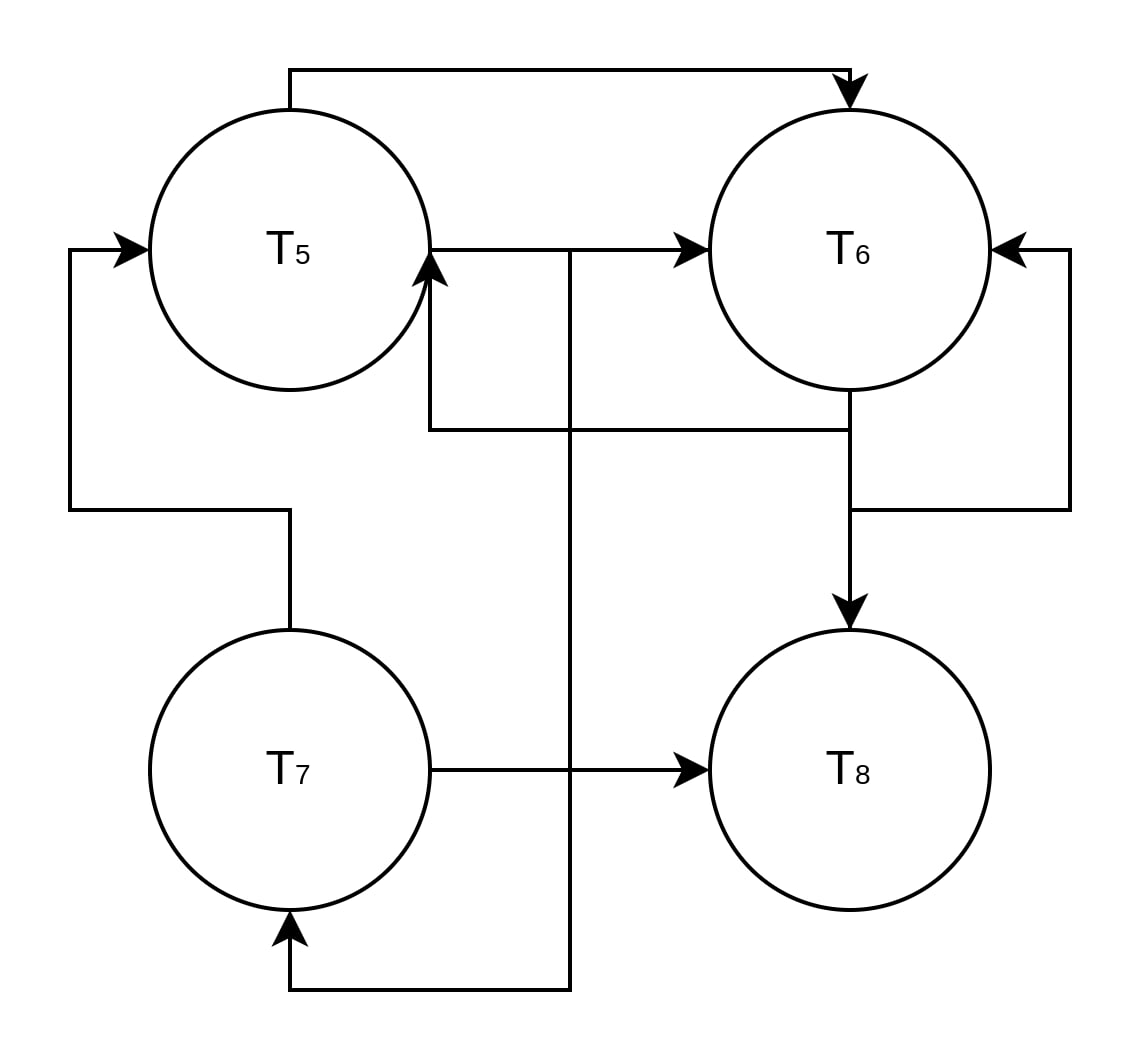
\includegraphics[width=0.3\textwidth]{umls/exp1_serializable_graph.jpg}
    \caption{گراف تراکنش‌ها و ایجاد ارتباطات حلقه دار}
    \label{fig: diagram}
\end{figure}

در این مثال برای حذف حلقه می‌تواند یکی یکی تراکنش‌های مورد نظر را بررسی کرد و در
صورت حذف یکی از تراکنش‌ها حلقه حذف شد می‌توان آن را نتیجه گرفت و اعلام کرد این
تراکنش‌ها باهم سازگارند و برخورد ایجاد نمی‌کنند. در نهایت سیستم DBM تصمیم به
اجرای تراکنش‌ها خواهد کرد.

\begin{figure}
    \centering
    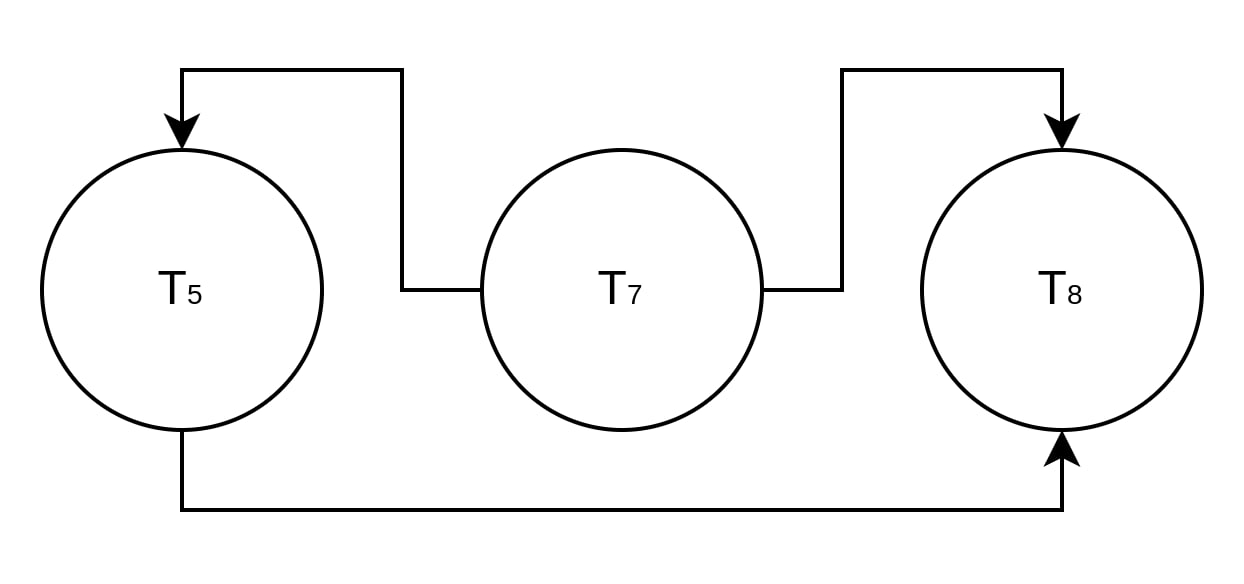
\includegraphics[width=0.3\textwidth]{umls/exp1_solved.jpg}
    \caption{تراکنش حذف شده و ایجاد گرافی بدون حلقه}
    \label{fig: diagram}
\end{figure}

\subsubsection{پی در پی پذیری در دید یا \lr{View equivalent}}

زمانی می‌گوییم پی در پی پذیری در دید برقرار است که نتایج \underline{یکسانی} در
سیستم DBM با یک زمان‌بندی پی در پی داشته باشیم.

سه قاعده اصلی پی در پی پذیری در دید:

\begin{enumerate}
    \item برای هر داده Q تراکنشی که در S مقدار اولیه داده‌ای Q  را می‌خواند در
    S' هم همان تراکنش اولیه مقدار Q را بخواند (خواندن‌های اولیه)
    \item برای هر داده‌ Q اگر $t_{i}$ در S داده‌ Q را از $t_{j}$ می‌خواند، در S'
    هم $t_{i}$ همان داده‌ را از $t_{j}$ بخواند. (خواندن‌های میانی)
    \item برای هر داده Q آخرین تراکنشی از S که روی Q می‌نویسد در S' هم همان
    تراکنش نوشتن پایانی را روی Q انجام دهد. (نوشتن‌های پایانی)
\end{enumerate}

نکته: یک زمانبندی پی در پی پذیر در دید است، هنگامی که معادل در دید با یک
زمانبندی پی در پی پذیر باشد که نتایج درستی را منعکس کند.

\subsubsection{مثال اول پی در پی پذیری در دید}

\begin{LTR}
    \begin{table}[h]
        \centering
        \begin{RTL}
            \caption{پی در پی پذیری در دید}
        \end{RTL}
        \begin{tabular}{c|c|c|c|c|c}
            $T_{5}$ & & & W(Q) & & \\ \hline
            $T_{6}$ & R(Q) & & & &  \\ \hline
            $T_{7}$ & & W(Q) & & & W(Q) \\ \hline
            $T_{8}$ & & & & R(Q) & \\
        \end{tabular}
    \end{table}
\end{LTR}

پی در پی پذیر در دید است چرا که فرایند خواندن اولیه و عملیات میانی و در نهایت
نوشتن پایانی را دارا می‌باشد.

\begin{LTR}
    $T_{6}$ > ....... > $T_{7}$

    $T_{6}$ > $T_{5}$ > $T_{8}$ > $T_{7}$
\end{LTR}

اما پی در پی پذیر در برخورد نیست چرا که بین تراکنش $T_{7}$ و $T_{8}$ یک حلقه
ایجاد می‌شود و می‌تواند عاملی در برخورد باشد.

\newpage

\subsubsection{مثال دوم پی در پی پذیری در دید}

\begin{LTR}
    \begin{table}[h]
        \centering
        \begin{RTL}
            \caption{پی در پی پذیری در دید}
        \end{RTL}
        \begin{tabular}{c|c|c|c}
            $T_{3}$ & R(Q) & & W(Q) C \\ \hline
            $T_{4}$ & & W(Q) C &  \\ \hline
            $T_{5}$ & & & W(Q) C \\
        \end{tabular}
    \end{table}
\end{LTR}

جواب: این مثال پی در پی پذیر در دید است:

\begin{LTR}
    $T_{3}$ > ....... > $T_{5}$
\end{LTR}

چرا که در $T_{3}$ خواندن‌های اولیه صورت گرفته، در $T_{4}$ و زمان میانی $T_{3}$
عملیات میانی نوشتن رخ داده است. در انتها در تراکنش $T_{5}$ مطابق با قانون پی در
پی پذیری در دید نوشتن پایانی انجام شده است.

اما پی در پی پذیر در برخورد نیست چرا که در میان تراکنش‌ها حلقه رخ داده است.

\begin{figure}
    \centering
    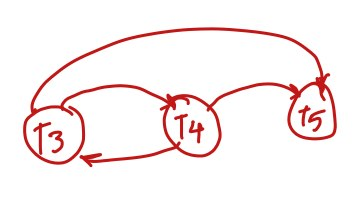
\includegraphics[width=0.4\textwidth]{umls/vsr_exp_2.jpg}
\end{figure}

\newpage

\subsubsection{نمادگزاری}

کامپیوتر چگونه پی در پی پذیری در دید را متوجه می‌شود؟ با استفاده از نمادگزاری
(خواندن از). برای یک زمانبندی، مجموعه‌ای از (خواندن از‌)ها را تشکیل می‌دهیم. این
مجموعه باید با مجموعه خواندن از‌ها در یک زمانبندی پی در پی دیگر یکسان باشد تا در
دید هم پی در پی پذیر باشد. در این روش مدت زمان اجرا \footnote{Runtime} برای
کامپیوتر طولانی است و اجرای آن برای کامپیوتر بهینه نیست.

مثال:

\begin{LTR}
$S = r_{2}(x), w_{2}(x), r_{1}(x), r_{1}(y), r_{2}(y), w_{2}(y), c_{1}, c_{2} $
\end{LTR}

\subsubsection*{بدست آوردن مرجع اصلی}

\begin{LTR}
$RF(S) = (T_{0}, x, T_{2}), (T_{2}, x, T_{1}), (T_{0}, y, T_{1}), (T_{0}, y, T_{2})$
\end{LTR}

\subsubsection*{بدست آوردن $T_{1} < T_{2}$}

در این مرحله ابتدا تراکنش‌های زمانبندی اول انجام می‌شود و سپس تراکنش‌های زمانبندی دوم:

\begin{LTR}
$T_{1} < T_{2}$ = $r_{1}(x), r_{1}(y), c_{1}, r_{2}(x), w_{2}(x), r_{2}(y), w_{2}(y), c_{2}$
\end{LTR}

بدست آوردن RF به وسیله ترتیب زمانبندی بالا:

\begin{LTR}
$RF(T_{1} < T_{2}) = (T_{0}, x, T_{1}), (T_{0}, y, T_{1}), (T_{0}, x, T_{2}), (T_{0}, y, T_{2})$
\end{LTR}

\subsubsection*{بدست آوردن $T_{2} < T_{1}$}

در این مرحله زمانبندی دوم در ابتدا و سپس زمانبندی اول بعد از آن اجرا می‌شود:

\begin{LTR}
$T_{2} < T_{1}$ = $r_{2}(x), w_{2}(x), r_{2}(y), w_{2}(y), c_{2}, r_{1}(x), r_{1}(y), c_{1}$
\end{LTR}

بدست آوردن RF به وسیله ترتیب زمانبندی جدید بالا:

\begin{LTR}
$RF(T_{2} < T_{1}) = (T_{0}, x, T_{2}), (T_{0}, y, T_{2}), (T_{0}, x, T_{1}), (T_{0}, y, T_{1})$
\end{LTR}

بعد از نوشتن عملیات بالا متوجه خواهید شد که هیچ کدام از $RF(T_{1} < T_{2})$ و
$RF(T_{2} < T_{1})$ با مرجع اصلی $RF(S)$ که در ابتدا نوشتیم برابر نیست.

\subsection*{یک زمانبندی ۲ شرط دارد که درست باشد:}

\begin{itemize}
    \item پی در پی پذیر باشد (قانون جامعیت در برخورد و دید برقرار باشد)
    \item ترمیم پذیر باشد
\end{itemize}

نکته: اگر یک زمانبندی پی در پی پذیر در برخورد باشد در دید هم پی در پی پذیر خواهد بود.

\section{ترمیم پذیری}

\subsection{مفهوم Rollback شدن}

اگر یک زمانبندی در میان اجرا Abort شود چون تراکنش‌های دیگر به آن وابسته هستند،
این تراکنش برای درست انجام شدن بایستی از اول انجام شود یا اصطلاحا Rollback صورت
گیرد.

\subsection{زمانبندی ترمیم پذیر یا \lr{Recoverable scheduling}}

زمانبندی را ترمیم پذیر می‌گوییم اگر $T_j$ از $T_i$ روی منبع اطلاعاتی خواندنی را
انجام می‌دهد که حتما به طور صحیح و کامل انجام شود. منظور از صحیح بودن آن است که
حتما تراکنش‌ها در زمانبندی Commit شده باشند. اما توجه شود که تراکنش قبلی بایستی
زودتر از تراکنش بعد خود Commit شده باشد.

\subsection*{مثال ۱: آیا زمانبندی زیر ترمیم پذیر است؟}

\begin{LTR}
    \begin{table}[h]
        \centering
        \begin{RTL}
            \caption{مثال ۱: بررسی ترمیم پذیری}
        \end{RTL}
        \begin{tabular}{c|c|c|c|c|c}
            $T_{1}$ & R(A) & W(A) & & R(B) & A \\ \hline
            $T_{2}$ & & & R(A) & & C \\
        \end{tabular}
    \end{table}
\end{LTR}

این زمانبندی ترمیم پذیر نیست چرا که درست نیست. زیرا در زمانبندی $T_{1}$ بعد از
انجام تراکنش عمل سقوط یا Abort اتفاق افتاده است و $T_{2}$ در حال خواندن مقدار از
منبعی از زمانبندی بالاتر خود است که تراکنش‌اش به دلیل \lr{Dirty Read} RollBack
خواهد شد و به صورت صحیح کامل نشده است.

\subsection*{مثال ۲: ترمیم پذیری زمانبندی زیر را بررسی کنید}

\begin{LTR}
    \begin{table}[h]
        \centering
        \begin{RTL}
            \caption{مثال ۲: بررسی ترمیم پذیری}
        \end{RTL}
        \begin{tabular}{c|c|c|c|c|c|c}
            $T_{1}$ & R(A) & W(A) & W(B) & C & \\ \hline
            $T_{2}$ & & & R(A) & W(A) & R(B) & C \\
        \end{tabular}
    \end{table}
\end{LTR}

این زمانبندی RC می‌باشد چرا که تراکنش‌ها به صورت صحیح انجام شد‌اند (عمل Commit
شدن در تراکنش‌ها وجود دارد). نکته مهم در این زمانبندی آن است که به دلیل وابسته
بودن عملیات تراکنش‌ها به یکدیگر ممکن است دائما در حال بررسی وجود Commit در
تراکنش‌ها باشیم تا زمانی عمل Abort رخ ندهد (اشاره به تراکنش دوم زمانی خواندن روی
منبع A صورت گرفته است). به همین دلیل زمانبندی ACA در اینجا تعریف خواهد شد. زمانی
تراکنش بالا می‌تواند ACA باشد که اولین خواندن دقیقا بعد از کامیت تراکنش اول صورت
گیرد.

\subsection{سقوط‌های آبشاری یا \lr{Cascading Aborts}}

در جدول ۱۲، دقیقا مانند مثال ۲، تمام تراکنش‌ها به همان شکل است. اما به جای کامیت
شدن در این جا تراکنش اول در نهایت سقوط می‌کند، هبا شکل دیگر ترمیم پذیر نخواهد
بود و با سقوط‌های آبشاری رو به رو است (اشاره به عملیات R(A) و R(B) که نوبتی سقط
می‌شوند).

\begin{LTR}
    \begin{table}[h]
        \centering
        \begin{RTL}
            \caption{بررسی سقوط‌های آبشاری در مثال ۲}
        \end{RTL}
        \scalebox{0.9}{
            \begin{tabular}{c|c|c|c|c|c|c}
                $T_{1}$ & R(A) & W(A) & W(B) & A & \\ \hline
                $T_{2}$ & & & R(A) & W(A) & R(B) & C \\
            \end{tabular}
        }
    \end{table}
\end{LTR}

\newpage

\subsection{\lr{Avoiding Cascading Aborts}}

در حقیقت فرایند زمانی فاقد سقوط آبشاری است; اگر $T_{j}$ از $T_{i}$ بخواند آنگاه
$T_{i}$ قبل از خواندن $T_{j}$ کامیت شده باشد. بطور کل به آن ACA می‌گویند که جز
تراکنش‌های ترمیم پذیر می‌باشد. به بیانی دیگر اگر قبل از اولین Read در تراکنش
دوم، در تراکنش اول کامیت صورت گرفته باشد آن زمانبندی ACA می‌باشد.

\begin{LTR}
    \begin{table}[h]
        \centering
        \begin{RTL}
            \caption{نمونه‌ای از فرایند ACA}
        \end{RTL}
        \scalebox{0.7}{
            \begin{tabular}{c|c|c|c|c|c|c|c|c|c}
                $T_{1}$ & R(A) & R(B) & W(A) & C & & & & & \\ \hline
                $T_{2}$ & & & & & R(A) & W(A) & C & & \\ \hline
                $T_{3}$ & & & & & & & & R(A) & C \\
            \end{tabular}
        }
    \end{table}
\end{LTR}

\subsection*{نکات}

\begin{itemize}
    \item در پی در پی پذیری تنها در مورد مشکلات همروندی صحبت می‌شد
    \item در زمانبندی‌های ACA هدف آن است که اول کامیت انجام شود و سپس خواندن
    منبع صورت گیرد در غیر این صورت زمان برای خواندن مقداری که تثبیط نشده است صرف
    می‌شود و زمان اصلی برای انجام فرایند‌های دیگر را از دست خواهیم داد.
    \item یکی از قوانین ترمیم پذیری عدم وجود سقوط‌های آبشاری است، پس اگر یک
    زمانبندی ACA باشد پس ترمیم پذیر می‌باشد.
\end{itemize}

\subsection*{سوال، زمانبندی زیر را از نظر ACA و RC بررسی کنید}

\begin{LTR}
    \begin{table}[h]
        \centering
        \begin{RTL}
            \caption{بررسی زمانبندی مثال ۴}
        \end{RTL}
        \scalebox{0.9}{
            \begin{tabular}{c|c|c|c|c|c|c|c}
                $T_{1}$ & R(A) & W(A) & W(B) & C & & & \\ \hline
                $T_{2}$ & & W(B) & W(C) & W(D) & R(A) & R(B) & C \\
            \end{tabular}
        }
    \end{table}
\end{LTR}

این زمانبندی ACA می‌باشد چرا که اولین Read در تراکنش $T_j$ دقیقا بعد از کامیت
تراکنش $T_i$ صورت گرفته است.

\subsection{زمانبندی‌های محض (سختگیرانه) یا Strict}

در دو تراکنش $T_{i}$ و $T_{j}$، اگر $T_{j}$ داده‌ای را پس از نوشتن $T_{i}$
بخواند یا بنویسد بایستی قبل از آن Commit صورت گرفته باشد.

\subsection*{مثال ۵: زمانبندی زیر را از نظر محض بودن، ترمیم پذیری و ACA بررسی کنید}

\begin{LTR}
    \begin{table}[h]
        \centering
        \begin{RTL}
            \caption{مثال ۵: بررسی تمام لایه‌های ترمیم پذیری}
        \end{RTL}
        \scalebox{0.9}{
            \begin{tabular}{c|c|c|c|c|c|c}
                $T_{1}$ & R(A) & R(B) & W(A) & & C & \\ \hline
                $T_{2}$ & & & & W(A) & W(B) & C \\ 
            \end{tabular}
        }
    \end{table}
\end{LTR}

\begin{itemize}
    \item زمانبندی بالا محض نیست، چرا که بعد از نوشتن در تراکنش $T_i$ بایستی
    کامیت گذاشته شود و سپس تراکنش $T_j$ می‌تواند خواندن و نوشتن خود را انجام
    دهد. در این مثال تراکنش دوم خواندن یا نوشتن خود را بعد از کامیت نوشتن تراکنش
    اول انجام نداده است.
    \item در این مثال به دلیل آنکه خواندنی بعد از کامیت صورت نگرفته (اشاره به
    قانون ACA می‌باشد) و تراکنش‌ها هر دو کامیت شده‌اند و یک زمانبندی صحیح
    می‌باشد، پس ترمیم پذیر می‌باشد.
\end{itemize}

نکته: سیستم DBM از یکسری پروتکل‌هایی برای \underline{پی در پی پذیری} و
\underline{ترمیم پذیری} استفاده می‌کند تا دیتابیس به شکل صحیح کار کند. (پیروی از
دو شرط اصلی)

\section{پروتکل‌های کنترل همروندی}

بعد از دیدن دستور، ۳ کار انجام می‌شود:

\begin{enumerate}
    \item اجرای دستور
    \item به تاخیر انداختن دستور (ممکن است به دلایلی وارد صف شود برای بدست آوردن
    قفل)
    \item نپذیرفتن دستور یا سقوط آن
\end{enumerate}

\subsection{پروتکل‌های مبتنی بر قفل}

در این نوع پروتکل واحدی به نام \lr{Lock Manager} تراکنش‌ها را بررسی می‌کند، اگر
ناسازگاری ww wr یا rw وجود نداشته باشد اجازه خواندن را به تراکنش می‌دهد و سپس
بعد از آن که تراکنش کارش تمام شد می‌تواند قفل را تحویل دهد تا تراکنش بعدی بتواند
عملیات قفل گذاری را انجام دهد.

\subsection*{قفل‌ها دو نوع هستند}

\begin{enumerate}
    \item قفل‌های دو حالته (دودویی): هیچ تفاوتی ندارد که تراکنش می‌خواهد بخواند
    یا بنویسد، به هر صورت قفل را اختصاص می‌دهد و در این فرایند هم تنها یک قفل
    برای هر دو عمل خواندن و نوشتن وجود دارد
    \item قفل‌های اشتراکی-انحصاری یا \lr{Shared Exclusive Lock}: از یک قفل برای
    خواندن (S) استفاده می‌کند و از قفل دیگر برای نوشتن (X)
\end{enumerate}

\subsection*{نکات}

\begin{itemize}
    \item مزیت قفل‌های اشتراکی-انحصاری در انجام تراکنش‌ها به صورت موازی است
    \item اگه قفل به حالت ناسازگار برسد آن تراکنش را به تاخیر می‌اندازد
    \item قفل گذاری روی داده‌های زیاد با Seed بالا همروندی را کاهش می‌دهد
    \item وقتی Seed کم باشد Overhead زمانی خواهیم داشت و پردازش گران است
    \item منظور از Seed در حقیقت منبعی است که می‌خواهیم روی آن قفل گذاری کنیم
    \item منابع مورد قفل گذاری می‌تواند یک ویژگی از جدول، یک جدول با رکورد‌های
    متفاوت و یا حتی یک \lr{OS Page Table} باشد
    \item قفل گذاری درست باعث می‌شود تا زمانبندی درست داشته باشیم
    \item زمانی که بر روی یک Table قفل می‌گذاریم، روی داده‌های بیشتری قفل گذاشته
    می‌شود و داده‌های بیشتری از دسترس خارج می‌شود که در نهایت همراه با همروندی
    کمتر است
    \item در قفل گذاری اشتراکی-انحصاری چندین تراکنش می‌توانند به طور همزمان قفل
    S را بدست آورند. زیرا حالت Read-Read پدید می‌آید  و حالت سازگاری است و مشکلی
    ایجاد نمی‌کند.
    \item حالت ناسازگار زمانی است که یک تراکنش بخواهد قفل S را بدست آورد و دیگری
    می‌خواهد قفل X را بدست آورد.
\end{itemize}

\subsection*{نوشتار}

\begin{itemize}
    \item $S_i(Q)$: دریافت قفل اشتراکی برای عملیات خواندن
    \item $X_i(Q)$: دریافت قفل انحصاری برای عملیات نوشتن
    \item $U_i(Q)$: آزادسازی قفل روی منبع Q
\end{itemize}

\subsection*{مثال ۱}

\begin{equation}
    S_{1} = R_{1}(A) W_{1}(A) A_{1} W_{2}(A) W_{2}(B) C
\end{equation}

\subsection*{پاسخ مثال ۱}

\begin{LTR}
    \centering
    $S_{1}$ = $S_{1}(A)$ $R_{1}(A)$ $X_{1}(A)$ $W_{1}(A)$ $U_{1}(A)$ $A_{1}$ $X_{2}(A)$ $W_{2}(A)$ $X_{2}(B)$ $W_{2}(B)$ $U_{2}(A)$ $U_{2}(B)$ $C$
\end{LTR}

\subsection*{مثال کلید اشتراکی-انحصاری}

\begin{LTR}
    \begin{table}[h]
        \centering
        \scalebox{0.8}{
            \begin{tabular}{c|c|c|c|c|c}
                $T_{3}$ & & & W(Q) & & \\ \hline
                $T_{4}$ & R(Q) & & & W(Q) & \\ \hline
                $T_{5}$ & & W(Q) & & & \\ \hline
                $T_{6}$ & & & & & R(Q) \\
            \end{tabular}
        }
    \end{table}
\end{LTR}

\subsection*{تبدیل جدول به سریال}

\begin{LTR}
    $R_{4}(Q)$ $W_{5}(Q)$ $W_{3}(Q)$ $W_{4}(Q)$ $R_{5}(Q)$
\end{LTR}

\subsection*{حل}

\begin{LTR}
    \centering
    $\rightarrow$ 
    $S_{4}(Q)$ $R_{4}(Q)$ 
    $X_{5}(Q)$ $X_{3}(Q)$
    $X_{4}(Q)$ $W_{4}(Q)$ $U_{4}(Q)$
    $W_{5}(Q)$ $U_{5}(Q)$
    $W_{3}(Q)$ $U_{3}(Q)$
    $S_{6}(Q)$ $R_{6}(Q)$ $U_{6}(Q)$
\end{LTR}

در این مسئله به دلیل وجود دو درخواست \footnote{\lr{Request}} در تراکنش $T_4$
ابتدا قفل به خواندن منبع Q اختصاص داده می‌شود ولی بعد از آن قفل آزاد نمی‌شود، تا
زمانی که این تراکنش به طور کامل کارش را انجام دهد و تمام شود. بعد از آن یکی یکی
تراکنش‌ها می‌توانند به درخواست‌هایشان برسند و عمل خواندن را از صف خارج کرده و
بعد از انجام موفقیت آمیز عملیات خواندن قفل را آزاد کنند.

\newpage

\subsection{بن بست و قحطی}

سوال: چه زمانی بن‌بست یا DeadLock رخ می‌دهد؟ زمانی که یک پردازه (تراکنش) منتظر
بدست آوردن قفل باشد. مهم‌ترین راهکار برای کم کردن بن‌بست حذف یا Abort تراکنش
باعث بن‌بست است.

\begin{LTR}
    \begin{table}[h]
        \begin{RTL}
            \caption{شکل کلی بن‌بست}
        \end{RTL}
        \centering
            \begin{tabular}{c|c}
                $T_1$ & $T_2$ \\ \hline
                \lr{Lock(A)} & \lr{Lock(B)} \\
                \lr{Lock(B)} & \lr{Lock(A)} \\
            \end{tabular}
    \end{table}
\end{LTR}

\begin{LTR}
    \begin{table}[h]
        \begin{RTL}
            \caption{نمونه‌ای از تراکنش‌هایی که به بن‌بست بر خورده‌اند}
        \end{RTL}
        \centering
            \begin{tabular}{c|c|c|c|c|c}
                $T_{3}$ & x(B) & w(B) & & & x(A) \\ \hline
                $T_{4}$ & & s(A) & r(A) & s(B) & \\
            \end{tabular}
    \end{table}
\end{LTR}

جدول بالا به دلیل ناسازگاری WR و RW به بن‌بست بر می‌خورد. چرا که در تراکنش
$T_{3}$ برای نوشتن روی منبع B قفل نوشتن گذاشته شده است ولی Unlock نشده است و
تراکنش $T_{4}$ نمی‌تواند قفل خواندن را روی منبع A بگذارد چرا که تراکنش $T_{3}$
هنوز قفل را آزاد نکرده است. در این حالت یک انتظار چرخشی یا \lr{Unlimited wating}
بین تراکنش‌ها رخ داده است که دائما منتظر آزاد سازی قفل یکدگیر هستند تا بتوانند
بقیه عملیات را انجام دهند. در $T_4$ قفل خواندن روی منبع A گذاشته می‌شود و بعد از
آن در خواست قفل گذاری را روی منبع B را دارد در حالی $T_3$ دقیقا روی منبع B عمل
نوشتن را انجام می‌دهد و قفل را رها نکرده است و در مقابل در ادامه همین تراکنش
درخواست نوشتن روی منبع A را دارد که در تراکنش $T_4$ درخواست آن داده شده ولی هیچ
قفلی آزاد نشده است. دلیل اصلی بن‌بست همین است.

بایستی در نظر داشت که با ساقط کردن یک تراکنش نمی‌توان به تنهایی مشکل بن‌بست را
حل کرد بلکه باعث ایجاد مشکل جدیدی به نام قحطی خواهد شد.  برای مثال یک تراکنش که
قصد زدن قفل x روی داده‌ای است منتظر دنباله‌ای از تراکنش‌ها بماند که همگی
می‌خواهند قفل s را روی همان منبع (داده) بزنند و این انتظار به پایان نرسد می‌گویم
در این حالت تراکنش تعریف قفل x روی منبع دچار قحطی شده است.

\begin{LTR}
    \begin{table}[h]
        \begin{RTL}
            \caption{قحطی}
        \end{RTL}
        \centering
            \begin{tabular}{c|c|c|c|c}
                $T_{1}$ & S(Q) & & & U(Q) \\ \hline
                $T_{2}$ & & X(Q) & & \\ \hline
                $T_{3}$ & & & S(Q) & \\ \hline
                $T_{4}$ & & & & S(Q) \\ \hline
                $...$ & & & & \\ 
            \end{tabular}
    \end{table}
\end{LTR}

در تراکنش‌های بالا به دلیل انتظار نامحدود ممکن است قحطی بین تراکنش‌های دیگر پیش
آید، به دلیل آنکه همه می‌خواهند روی یک منبع عملیاتی را انجام دهند که در تراکنش
اول قفل خواندن در دست است و تراکنش‌های دیگر باید منتظر آزاد سازی آن باشند.

\newpage

\subsection{پروتکل‌های قفل دو مرحله‌ای 2PL}

برای توضیح این پروتکل‌ها تراکنش‌های زیر را در نظر بگیرید:

\begin{LTR}
    \begin{table}[h]
        \begin{RTL}
            \caption{زمانبندی $S_{5}$}
        \end{RTL}
        \centering
        \scalebox{0.83}{
            \begin{tabular}{c|ccccccccccccccc}
                $T_{1}$ & x(A) & Dec(A, amount) & w(A) & u(A) & & & & & & & x(B) & Inc(B, amount) & w(B) & u(B) &  \\ \hline
                $T_{2}$ & & & & & s(A) & r(A) & s(B) & r(B) & Dis(A+B) & u(A) & u(B) & & & &  \\
            \end{tabular}
        }
    \end{table}
\end{LTR}

در جدول ۱۶، شما تراکنش‌هایی را می‌بینید که در حال کم کردن از یک منبع و اضافه
کردن آن مقدار به منبع دیگری هستند. ولی این تراکنش‌ها صحیح نیستند و دیتابیس
نمی‌تواند به درستی کار کند چرا که با بازیابی ناسازگار رو به رو است. با توجه به
تراکنش $T_{2}$ می‌توان دریافت که بعد از قفل گذاری روی منبع A برای خواندن، سعی در
قفل گذاری رو منبع B دارد که اصلا معتبر نیست. زیرا در تراکنش $T_{1}$ هیچ عملیات
یا حتی قفل گذاری روی منبع B انجام نشده است که الان سعی در خواندن آن دارد. پس با
بازیابی ناهمگام یا \lr{Inconsistent retrieval} رو به رو خواهد بود و باید از یک
پروتکل قفل گذاری مناسب جهت این کار استفاده کند.

\subsection*{نکته}

اگر زمابندی پی در پی پذیر در برخورد باشد آنگاه تمام مشکلات مربوط به
همروندی تراکنش‌ها برطرف خواهد شد.

\subsection{مراحلی که در فرایند پروتکل 2PL برای قفل گذاری صورت می‌گیرد}

\subsection*{مرحله اول - مرحله رشد یا \lr{Growing}}

در این مرحله تراکنش می‌تواند قفل گذاری کند (احتمال انجام کار را دارد)، اما
نمی‌تواند قفل را آزاد کند.

\subsubsection*{مرحله دوم - مرحله عقب نشینی یا \lr{Shrinking}}

در این مرحله تراکنش می‌تواند قفل را آزاد کند (احتمال انجام کار دارد)، اما
نمی‌تواند روی منبعی قفل گذاری جدیدی را انجام دهد.

\newpage

\subsection{پروتکل B2PL یا \lr{Basic Two Phase Locking}}

در این مرحله، تراکنش‌ها شروع به قفل گذاری منابع برای انجام عملیات خود می‌کنند به
محض اینکه یکی از تراکنش‌ها قفلی را آزاد کند وارد مرحله دوم یا Shrinking خواهد شد
و از این بعد نمی‌تواند هیچ قفل گذاری را انجام دهد.


\begin{LTR}
    \begin{table}[h]
        \begin{RTL}
            \caption{زمانبندی $S_{6}$}
        \end{RTL}
        \centering
        \scalebox{0.73}{
            \begin{tabular}{c|cccccccccccccccc}
                $T_{1}$ & X(A) & Dec(A, amount) & W(A) & X(B) & Inc(B, amount) & U(a) & & & W(B) & U(B) & & & & & &  \\ \hline
                $T_{2}$ & & & & & & & S(A) & R(A) & & & S(B) & R(B) & Dis(A+B) & U(A) & U(B) &   \\
            \end{tabular}
        }
    \end{table}
\end{LTR}

این پروتکل قفل گذاری ترمیم پذیر نخواهد بود چرا که مشکل بن‌بست و سقوط‌های آبشاری
را دارد. برای رفع این مشکلات پروتکل دیگری به نام C2PL یا قفل گذاری محافظه کارانه
را معرفی کردند.

\subsection{قفل گذاری C2PL یا \lr{Conservative Two Phase Locking}}

در این پروتکل قبل از اجرای هر دستور و عملیاتی، تراکنش‌ها بایستی قفل‌های مورد
نیاز را از قبل گرفته باشند اگر موفق نشد دوباره در صف قرار می‌گیرد (تا اینکه
قفل‌های قبلی باز شوند و بتواند قفل جدیدی را تعریف کند).

\begin{LTR}
    \begin{table}[h]
        \begin{RTL}
            \caption{زمانبندی $S_{7}$}
        \end{RTL}
        \centering
        \scalebox{0.73}{
            \begin{tabular}{c|ccccccccccccccccc}
                $T_{1}$ & X(A) & X(B) & Dec(A, amount) & W(A) & Inc(B, amount) & W(B) & U(A) & & & U(B) & C & & & & & & \\ \hline
                $T_{2}$ & & & & & & & & S(A) & R(A) & & & S(B) & R(B) & U(A) & Disp(A+B) & U(B) & C \\
            \end{tabular}
        }
    \end{table}
\end{LTR}

مهم‌ترین مشکلات این روش پایین آمدن سطح سرعت همروندی و نیاز به دانستن مجموعه
قفل‌های مورد نیاز هر تراکنش قبل از شروع اجرای دستورات می‌باشد. امکان بن‌بست در
این روش از بین می‌رود اما باز هم ترمیم پذیر نخواهد بود فلذا می‌تواند باعث رخ
دادن سقوط آبشاری شود. استفاده از این پروتکل گران است چرا که برای تضمین عدم وقوع
بن‌بست، سرعت و کارایی همروندی را تا حد چشمگیری کاهش می‌دهد در حالی که در دنیای
واقعی احتمال بروز بن‌بست آنقدر زیاد نمی‌باشد.

\subsection{پروتکل S2PL یا \lr{Strict Two Phase Locking}}

به طور کلی در این پروتکل بعد از قفل گذاری‌ها، ابتدا تراکنش بایستی کامیت یا Abort
شود و سپس قفل‌هایی که در اختیار دارد را آزاد می‌کند. قفل‌های خواندن می‌تواند کمی
زودتر بعد از آخرین دستور تراکنش یا قبل از کامیت یا Abort باز شوند وگرنه در بقیه
عملیات شبیه B2PL عمل می‌کند. اگرچه این پروتکل کمی سختگیرانه عمل می‌کند و شاید
بسیاری از زمانبندی‌ها که در واقع درست هستند را به دلیل احتمال بروز مشکل نپذیرد،
اما به عنوان یکی از بهترین گزینه‌ها در اکثر سیستم‌های دیتابیسی مورد استفاده قرار
گرفته است. مزیت اصلی این پروتکل که آنرا به پرکاربردترین و بهترین گزینه تبدیل
کرده است، تمضین پی در پی پذیری و ترمیم پذیری است. از مزیت دیگر این پروتکل
می‌توان به کم کردن پیام‌ها در بانک‌های اطلاعاتی نامتمرکز اشاره کرد زیرا نیازی به
پیام‌های باز کردن قفل ندارد.

\begin{LTR}
    \begin{table}[h]
        \begin{RTL}
            \caption{زمانبندی $S_{8}$}
        \end{RTL}
        \centering
        \scalebox{0.73}{
            \begin{tabular}{c|ccccccccccccccccc}
                $T_{1}$ & X(A) & Dec(A, amount) & W(A) & X(B) & Inc(B, amount) & W(B) & \textbf{C} & U(A) & & U(B) & & & & & & & \\ \hline
                $T_{2}$ & & & & & & & & & S(A) & & R(A) & S(B) & R(B) & Disp(A+B) & \textbf{C} & U(A) & U(B)  \\
            \end{tabular}
        }
    \end{table}
\end{LTR}

\subsection*{نکات و بررسی SS2PL یا R2PL}

\begin{enumerate}
    \item این پروتکل همانطور که از نامش پیداست (\lr{Strong Strict}) سختگیرانه‌تر
    از S2PL می‌باشد و معمولا استفاده نمی‌شود.
    \item در این پروتکل قفل‌های خواندن و نوشتن یا S و X باید بعد از Abort یا
    Commit آزاد شوند.
\end{enumerate}

\subsection{پروتکل SC2PL}

این پروتکل ترکیبی از دو پروتکل S2PL و C2PL برای بهروری و کارایی بیشتر است. در
این پروتکل بن‌بست و گرسنگی و سقوط آبشاری وجود ندارد! عملکرد این پروتکل با خواندن
دو پروتکل ترکیبی آن حاصل می‌شود. اما کمترین میزان همروندی را خواهد داشت.

\begin{LTR}
    \begin{table}[h]
        \begin{RTL}
            \caption{زمانبندی $S_{9}$}
        \end{RTL}
        \centering
        \scalebox{0.73}{
            \begin{tabular}{c|ccccccccccccccccc}
                $T_{1}$ & X(A) & X(B) & Dec(A, amount) & W(A) & Inc(B, amount) & W(B) & \textbf{C} & U(A) & & U(B) & & & & & & & \\ \hline
                $T_{2}$ & & & & & & & & & S(A) & & S(B) & R(A) & R(B) & Disp(A+B) & \textbf{C} & U(A) & U(B) \\
            \end{tabular}
        }
    \end{table}
\end{LTR}

\subsection*{مثال ۱}

معادل زمانبندی زیر را یکبار با قفل باینری و یکبار با قفل S/X و رعایت پروتکل B2PL
بنویسید:

\begin{LTR}
    \begin{table}[h]
        \begin{RTL}
            \caption{زمانبندی $S_{10}$}
        \end{RTL}
        \centering
        \scalebox{0.87}{
            \begin{tabular}{c|c|c|c|c|c|c|c|c|c}
                $T_{1}$ & R(Q) & & & & W(Q) & & & & \\ \hline
                $T_{2}$ & & R(A) & & & & & R(Q) & & \\ \hline
                $T_{3}$ & & & R(Q) & & & R(P) & & W(P) & \\ \hline
                $T_{4}$ & & & & W(Q) &  & & & & W(A) \\
            \end{tabular}
        }
    \end{table}
\end{LTR}

\subsection*{قفل باینری}

\begin{LTR}
\centering
$L_1(Q)R_1(Q)L_2(A)R_2(A)[L_3(Q)L_4(Q)]W_1(Q)U_1(Q)C_1R_3(Q)L_3(P)R_3(P)[L_2(Q)]$

$W_3(P)U_3(Q)U_3(P)C_3[W_4(Q)]L_4(A)[Deadlock]$
\end{LTR}

\subsection*{قفل S/X}

\begin{LTR}
\centering
$S_10 = S_1^*(Q)R_1(Q) S_2^*(A)R_2(A) S_3^*(Q)R_3(Q) [X_4(Q)][X_1(Q)]S_3^*(P)R_3(P) S_2^*(Q)R_2(Q) U_2(A)U_2(Q)C2$

$X_3(P)W_3(P) U_3(Q)U_3(P)C_3W_1(Q)U_1(Q)C_1W_4(Q)X_4(A)W_4(A)U_4(Q)U_4(A)C_4$
\end{LTR}

\subsubsection*{نکته}

در این روش قفل گذاری به دلیل وجود ناسازگاری RW یا WR نمی‌توان به نوشتن‌ها به
دلیل خواندن‌های قبلی روی منبع مشترک قفل اختصاص داد. بلکه بایستی کار خواندن‌ها
روی آن منبع مشترک به طور کامل تمام شود تا قفل را آزاد کند و سپس به نوشتن‌ها
اختصاص یابد.

\subsection*{مثال ۲}

همین تمرین را با پروتکل‌های C2PL S2PL و SC2PL انجام دهید.

\newpage

\section{پروتکل‌های مبتنی بر مهر زمانی \lr{Timestamp}}

مهم‌ترین کاربرد را در دیتابیس‌های توزیع شده دارد. هر تراکنش به محض ورود، یک مهر
زمانی تصاعدی به آن داده می‌شود. مهر زمانی تراکنش $T_i$ را به صورت $TS(T_i)$
نمایش می‌دهیم. مسلم است که برای دو تراکنش $T_i$ و $T_j$ که $T_j$ دیرتر وارد
سیستم شده است به صورت $TS(T_i) < TS(T_j)$ می‌باشد. بر این اساس، پروتکل مبتنی بر
مهر زمانی، تراکنش‌ها را به  ترتیب مهر زمانی آن ها به صورت پی در پی پذیر اجرا
می‌کند. اکنون که این برگه نوشته می‌شود timestamp آن به صورت \lr{1703397265}
می‌باشد.  بعد از آن دوباره اقدام به تولید یک زمان دیگر کردیم که به مقدار
\lr{1703397306} رسیدیم. با مقایسه این دو زمان می‌توانید دریابید که زمان اول
زودتر از زمان دوم نوشته شده است پس کوچکتر می‌باشد اما سن آن چند ثانیه بیشتر
می‌باشد یا به طور کلی به شکل زیر آن را می‌نویسم:

\begin{equation}
    1703397265 < 1703397306 
\end{equation}

\subsection*{نکته}

برای هر داده Q مهر زمانی خواندن و نوشتن آن به صورت زیر تعریف می‌شود:

\begin{itemize}
    \item زمان $W-TS(Q)$: مهر زمانی نوشتن داده Q که برابر است با بزرگترین مهر
    زمانی تراکنشی که به طور موفقیت آمیز روی Q نوشته است.
    \item زمان $R-TS(Q)$: مهر زمانی خواندن Q که برابر است با بزرگ ترین مهر زمانی
    تراکنشی که به طور موفقیت آمیز Q را خوانده است.
\end{itemize}

\subsection{قواعد}

این قواعد تضمین می‌کنند که دستورات خواندن و نوشتن با هم برخورد دارند و به ترتیب
مهر زمانی اجرا خواهند شد و زمانبندی‌های مربوطه پی در پی پذیر هستند.

\subsubsection{قاعده خواندن}

تراکنش $T_i$ شامل یک دستور Read(Q) است آنگاه:

\begin{enumerate}
    \item اگر $TS(T_i) < W-TS(Q)$ آنگاه تراکنش $T_i$ داده‌ای را می‌خواند که
    مقدارش انگار بعداً نوشته می‌شود. پس در این صورت با دستور خواندن تراکنش
    موافقت نمی‌شود و تراکنش رد (Reject) خواهد شد.
    \begin{LTR}
        \begin{table}[h]
            \begin{RTL}
                \caption{بررسی مهر زمانی در قاعده خواندن}
            \end{RTL}
            \centering
            \scalebox{0.87}{
                \begin{tabular}{c|cc}
                    $T_{1}$ & R(Q) & \\ \hline
                    $T_{2}$ & & W(Q) \\
                \end{tabular}
            }
        \end{table}
    \end{LTR}

    \item اگر $TS(T_i) >= W-TS(Q)$ آنگاه دستور خواندن تراکنش $T_i$ اجرا می‌شود و
    مهر زمانی خواندن Q با \lr{Max} بین مهر زمانی تراکنش $T_i$ و مهر زمانی خواندن
    Q مقداردهی می‌شود

    \begin{LTR}
        \begin{table}[h]
            \begin{RTL}
                \caption{بررسی مهر زمانی در قاعده خواندن}
            \end{RTL}
            \centering
            \scalebox{0.87}{
                \begin{tabular}{c|cc}
                    $T_{1}$ & W(Q) & \\ \hline
                    $T_{2}$ & & R(Q) \\
                \end{tabular}
            }
        \end{table}
    \end{LTR}

\end{enumerate}

\subsubsection*{منظور از Reject شدن در چیست؟}

وقتی می‌گوییم تراکنش Reject یا رد خواهد شد یعنی آنکه یا ممکن است منتظر اجرا
(Wait) بماند یا ساقط و مجددا اجرا (\lr{Abort and Rollback}) شود.

\subsubsection{قاعده نوشتن}

تراکنش $T_i$ شامل یک دستور Write(Q) است آنگاه:

\begin{enumerate}
    \item اگر $TS(T_i) < W-TS(Q) || TS(T_i) < R-TS(Q)$ باشد، آنگاه با دستور
    نوشتن تراکنش موافقت نمی‌شود و تراکنش $T_i$ رد یا Reject می‌شود (اشاره به
    ناسازگاری \lr{WW} و \lr{WR}).

    \item در غیر این صورت دستور نوشتن اجرا می‌شود و مهر زمانی نوشتن Q نیز با
    $TS(T_i)$ مقداردهی می‌شود (اگر به صورت برعکس مورد بالا باشد یعنی: $TS(T_i) >
    R-TS(Q) \&\& TS(T_i) > W-TS(Q) $)
\end{enumerate}

\subsubsection*{نکات}

\begin{itemize}
    \item اگر هیچ تراکنشی به حالت رد شدن نرود این پروتکل‌ها فاقد بن‌بست خواهند
    بود اما ممکن است ترمیم پذیر نباشد.

    \item گراف زمانبندی‌های مهر زمانی همواره پی در پی پذیر خواهند بود چرا که
    همواره زمان در حال تغییر است و از زمان کوچک (سن بالاتر) به سمت زمان بزرگ‌تر
    (سن کوچک‌تر) می‌رود و هیچ دوری تشکیل نمی‌شود.
\end{itemize}

\subsection*{مثال}

زمانبندی زیر را با پروتکل‌های S2PL و C2PL و مهر زمانی بنویسید.

\begin{LTR}
    \centering
    $R_1(A),R_2(B),R_1(B),W_1(B),R_3(C),W_2(A)$
\end{LTR}

\newpage

\section{روش‌های مدیریت بن‌بست}

همان طور که در بخش‌های قبلی نوشته شد، زمانی سیستم دچار بن‌بست می‌شود که تو
تراکنش قفل‌های یکدیگر را درخواست کرده باشند یا اینکه مجموعه‌ای از تراکنش‌ها برای
همیشه منتظر یکدیگر برای دریافت قفل باشند.

مهم‌ترین استراتژی‌های مدیریت بن‌بست موارد زیر می‌باشد

\subsection{چشم پوشی یا \lr{Ignore}}

در عمل اتفاق بن‌بست بسیار پایین و هزینه مقاله با آن گران است به همین خاطر یکی از
روش‌های مقابله با بن‌بست چشم پوشی کردن از آن است.  یک نوع وابستگی خارج از سطح
سیستم است که معمولا برنامه‌نویس یا مدیر سیستم (یا هر عامل دیگری) مسئول برطرف
کردن آن است.

\subsection{فرصت یا \lr{Timeout}}

تراکنشی که به حالت انتظار می‌رود، فقط برای مدت زمان معینی منتظر می‌ماند (اگر
سرویس نگرفت) پس از آن ساقط می‌شود و دوباره بایستی درخواست اجرایش انجام شود. این
روش یک روش ساده است که از بن‌بست جلوگیری می‌کند ولی امکان بروز قحطی در آن زیاد
است. مقدار timeout در سیستم کار مشکل و پیچیده‌ای است.

\subsection{پیشگیری یا \lr{Prevention}}

استفاده از پروتکل‌هایی که نبود بن‌بست را تضمین می‌کنند، مانند:

\begin{itemize}
    \item پروتکل SC2PL
    \item پروتکل C2PL
    \item استفاده از timestamp به شرطی که رد شدن در آن به معنای انتظار نباشد
    بلکه به معنای Rollback باشد.
\end{itemize}

\subsection{اجتناب یا \lr{Avoidance}}

در این روش بن‌بست تشخیص داده می‌شود و از اجرای دستوری که موجب آن شود جلوگیری به
عمل می‌آورد. در این روش از مهر زمانی مخصوص بن‌بست استفاده می‌کنیم. دو حالت دارد:

\begin{itemize}
    \item روش \lr{Wait die}: تراکنش پیرتر (با timestamp کمتر) منتظر می‌ماند که
    تراکنش جوان‌تر قفل مربوطه را آزاد کند. در مقابل تراکنش جوان‌تر هرگز منتظر
    نمی‌ماند بلکه ساقط می‌شود (می‌میرد). ممکن است یک تراکنش چندین بار بمیرد.
    
    \item روش \lr{Wound wait}: در این روش تراکنش پیرتر به جای انتظار تراکنش
    جوان‌تر را می‌کشد (kill) ولی تراکنش جوان‌تر منتظر تراکنش پیرتر می‌ماند. در
    این روش برخلاف روش \lr{Wait die} تراکنش پیرتر اولویت بالاتری دارد و با گشتن
    تراکنش جوان فرایند اجرا را به قبضه خود در می‌آورد.
\end{itemize}

\subsection*{نکته}

تعداد تراکنش‌های جوان‌تر که منتظر هستند بیشتر از تراکنش‌هایی با مهر زمانی پیرتر
است. در هر دو روش گفته شده، تراکنشی که ساقط می‌شود با همان مهر زمانی اصلی خود
(مثلا ثانیه ۱۰ وارد شده و زمان کنونی ثانیه ۱۰۰ است پس ۱۰ از ۱۰۰ پیرتر خواهد بود)
آغاز به کار مجدد می‌کند که به همین دلیل باعث می‌شود تراکنش جوان پس از چند بار
مردن، بالاخره پیر شود و بتواند تراکنش را قبضه کند و از بروز قحطی جلوگیری کند.

\subsection{تشخیص و رفع بن‌بست یا \lr{Detection and resolve}}

در این روش از گراف انتظار استفاده می‌کنیم. به ازای تمام حالاتی‌ که بین
تراکنش‌های $T_i$ و $T_j$ حالت‌های ww و WR و RW رخ می‌دهد را یک یال می‌کشیم. اگر
در گراف دور ایجاد شود بن‌بست رخ داده است. در این حالت باید تراکنشی که تعداد
دور‌های بیشتری دارد را kill کنیم تا دور از بین برود یا اینکه تشخیص دهیم که کدام
تراکنش کار بیشتری انجام داده است که اگر اکثر فرایندش را انجام داده در پایان کار
آن را kill کنیم.

\newpage

\section{واحد مدیریت ترمیم و الگوریتم‌ها}

\subsection*{دو تراکنش زیر چه قوانینی را تقض کرده‌اند؟ توضیح دهید}

\begin{LTR}
    \begin{table}[h]
        \begin{RTL}
        \end{RTL}
        \centering
            \begin{tabular}{c|c}
                $T_1$ & $T_2$ \\ \hline
                : & : \\
                : & : \\
                : & : \\
                : & : \\
                Failure & : \\
                : & Commit \\
                : & Failure
            \end{tabular}
    \end{table}
\end{LTR}

در تراکنش $T_1$ قانون Atomicity رعایت نشده است، چرا که حین اجرا به مشکل بر خورده
و تراکنش اول به پایان نرسیده است. یکی از مهم‌ترین قوانین ACID بخش Atomicity است
که تراکنش یا باید کامل انجام شود که کامیت شود یا نهایتا سقوط کند.

در تراکنش $T_2$ قانون Duribility رعایت نشده است. یعنی تراکنش به صورت کامل انجام
شده است و حتی کامیت هم صورت گرفته اما در حافظه و یا قسمتی که مربوط به ثبت داده
این تراکنش است منعکس نشده است.

\subsection{انواع خطا‌های مربوط به سیستم دیتابیس}

\subsubsection{خطا‌های تراکنشی}

\begin{enumerate}
    \item خطای منطقی: تراکنش با توجه به قوانینی که برای آن تعریف کردیم، اشتباه
    انجام شود، مانند خطای تقسیم بر صفر. این نوع خطا بر روی کل دیتابیس تاثیر گذار
    نیست
    \item خطای سیستمی: مانند Kill شدن تراکنش‌ها به هر دلیلی
\end{enumerate}

\subsubsection{خطا‌های سیستمی}

خطای سیستمی می‌تواند مربوط به سخت‌افزار و نرم‌افزار شود، برای مثال سیستم هنگ
کرده باشد، رم پر شده باشد یا از نظر سخت‌افزاری مشکلی برای آن پیش آمده باشد.

\subsubsection{خطای رسانه‌ای}

خرابی حافظه (دیسک) که می‌تواند سخت‌افزاری هم باشد اما بخش بسیار مهم یک سیستم
دیتابیسی را شامل می‌شود که می‌تواند روی همه داده‌ها تاثیر گذار باشد.

\subsubsection*{یادآوری}

واحد مدیریت همروندی مسئول برقرار خاصیت Isolation است در حالی که واحد مدیریت
ترمیم مسئول انجام شدن کامل تراکنش‌ها و خاصیت ماندگاری است.

\subsection{روال دسترسی به داده‌ها برای انجام تراکنش}

% @startuml
% package Storage {
%   package Buffer {
%     [AB] as "A"
%     [BB] as "B"
%   }
%   package TransactionsA {
%     [A1] as "A"
%     [B1] as "B"
%   }
%   package TransactionsB {
%     [An] as "An"
%   }
% }

% package Media {
%    database DB {
%     [A]
%     [B]
%   }
% }

% A --> Buffer: "Input()"
% Buffer --> B: "Output()"

% A1 --> Buffer: "Read()"
% B1 <-- Buffer: "Write()"
% @enduml

\begin{figure}
    \centering
    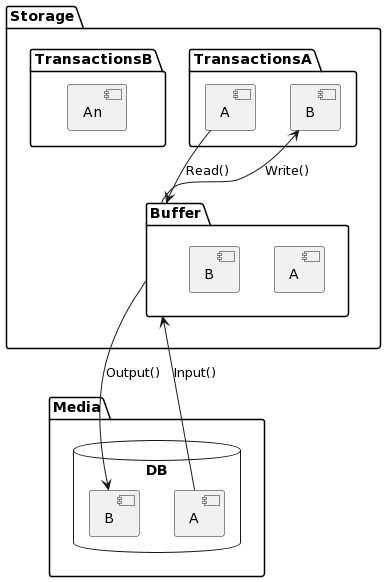
\includegraphics[width=0.3\textwidth]{umls/media.png}
    \caption{روال دسترسی به داده برای انجام تراکنش}
    \label{fig:media}
\end{figure}

داده‌های دیتابیس روی رسانه‌ها قرار دارند که به منظور پردازش آنها توسط
تراکنش‌ها،‌باید به طور موقت به بخشی از حافظه اصلی منتقل شوند که آنرا بافر
\footnote{Buffer} می‌گوییم. آوردن داده از دیسک به بافر و بازگرداندن نتایج از
بافر به دیسک (معمولا به صورت بلاک‌های حافظه) توسط عملگر‌هایی (توابع) انجام
می‌شود که \lr{input()} و \lr{output()} نامیده می‌شود. هر تراکنشی که می‌خواهد با
داده‌ای کار کند، یک کپی از آن داده در بافر را در ناحیه کاری \footnote{Workarea}
خاص خود می‌برد و دسترسی‌های بعدی آن تراکنش روی کپی محلی اش انجام می‌شود و پس از
اتمام کار، این کپی محلی به بافر منقل می‌شود. باز هم برای این منظور نیاز به
عملگرذهایی داریم که آنها را به ترتیب \lr{Read()}و \lr{Write()} می‌نامیم. شکل
\ref{fig:media} این موضوع را نشان می‌دهد. به طور خلاصه، خواندن و نوشتن روی
داده‌ها در workarea رخ می‌دهد که بعد از آن انتقال داده‌ها اول روی حافظه اصلی و
منطقی (بافر) صورت می‌گیرد و در نهایت از حافظه اصلی به حافظه جانبی و یا دیسک منقل
می‌شود.

\subsection*{نکته}

اگر داده در بافر حضور نداشته باشد درخواست خواندن را به دیسک ارسال می‌کند.

\subsection{الگوریتم‌های ترمیم}

الگوریتم‌های ترمیم برای حفظ جامیت و پایداری شامل دو مرحله می‌شوند، (به طور کلی
همان بک‌آپ و ری‌استور کردن داده‌ها می‌باشد)

\subsubsection{مرحله اول}

در این مرحله، حین اجرای تراکنش اطلاعاتی برای ترمیم نیاز است را در جایی ثبت
می‌کند.

\subsubsection{مرحله دوم}

در این مرحله، بعد از آنکه سیستم بالا آمد و وضعیت کلی مناسبی داشت اطلاعاتی که در
مرحله قبل ثبت شده در این مرحله خوانده می‌شود تا خواص Atomicity و Duribility
برقرار باشد.

\subsection*{طبق خاصیت Duribility}

اثرات تراکنشی که انجام شده باید دائمی و همیشگی باشد.


\subsection*{طبق خاصیت Atomicity}

تراکنشی که نیمه کاره متوقف شده است نباید هیچ اثری در دیتابیس داشته باشد.

\subsection{عملیات Redo}

زمانی عملیات را Redo می‌کنیم که تراکنش به صورت کامل کامیت شده و در انعکاس
اطلاعات در حافظه به مشکل خورده است (توجه شود تمام فرایند از اول انجام می‌شود).

\subsection{عملیات Undo}

زمانی عملیات را Undo می‌کنیم که خاصیت جامیعت نقض شده باشد. برای مثال تراکنش ساقط
شده باشد. به خاطر همین دستورات را مرحله به مرحله خنثی می‌کنیم (عملیات Undo از
پایین به بالا انجام می‌شود. از آخرین دستور تا اولین دستور).

\subsection{رویکرد‌های الگوریتم ترمیم}

\begin{itemize}
    \item کارنامه \footnote{Log}
    \item رونوشت
\end{itemize}

\subsection{رویکرد کارنامه}


\end{document}